% Created 2024-01-08 Mon 13:50
% Intended LaTeX compiler: pdflatex
\documentclass[svgnames, 11pt, lettersize]{article}
\usepackage[utf8]{inputenc}
\usepackage{lmodern}
\usepackage[T1]{fontenc}
\usepackage[top=1in, bottom=1.in, left=1in, right=1in]{geometry}
\usepackage{graphicx}
\usepackage{longtable}
\usepackage{float}
\usepackage{wrapfig}
\usepackage{rotating}
\usepackage[normalem]{ulem}
\usepackage{amsmath}
\usepackage{textcomp}
\usepackage{marvosym}
\usepackage{wasysym}
\usepackage{amssymb}
\usepackage{amsmath}
\usepackage[theorems, skins]{tcolorbox}
\usepackage[version=3]{mhchem}
\usepackage[numbers,super,sort&compress]{natbib}
\usepackage{natmove}
\usepackage{url}
\usepackage[cache=false]{minted}
\usepackage[strings]{underscore}
\usepackage[linktocpage,pdfstartview=FitH,colorlinks,
linkcolor=blue,anchorcolor=blue,
citecolor=blue,filecolor=blue,menucolor=blue,urlcolor=blue]{hyperref}
\usepackage{attachfile}
\usepackage{setspace}
\usepackage{breakurl}
\usepackage{Newuli}
\usepackage{uli-german-paragraphs}
\usepackage{makeidx}
\author{Uli Wortmann}
\date{\today}
\title{}
\begin{document}

\section{ESS245 Computational Geology: Interacting with Jupyter 2}
\label{sec:org2990cfc}
Since Jupyter notebooks will be the primary tool we use in this
course, and the dominant format for your assignment submissions, we
will explore their use in greater detail in the following.

A Jupyter notebook has three principal elements see Fig.\ref{nbexample}

\begin{enumerate}
\item Text areas (often referred to as cells). You can edit these text2 cells.
\item Code blocks (or code cells). These contain computer code that can
be executed. You can edit and execute these cells.
\item Result Blocks, which contain the output produced by a code
block. Results blocks cannot be edited. However, you can select and
copy them.
\end{enumerate}
\begin{figure}[htbp]
\centering
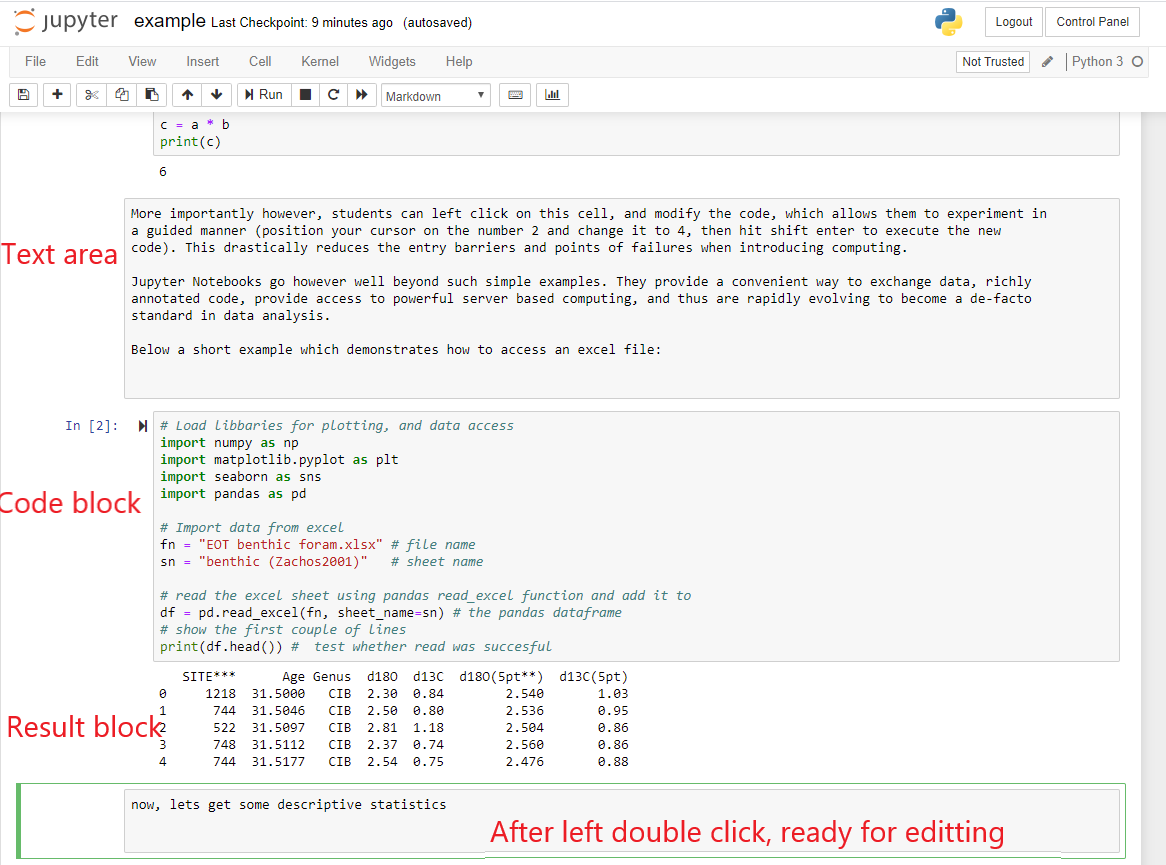
\includegraphics[width=0.7\textwidth]{./Tianshi/TL-fig-003.png}
\caption{\label{nbexample}An example of a Jupyter notebook (.ipynb file) including text areas, code blocks and result blocks. After double left click on the cell, the cell will be ready for editing (and the bar will change to green)}
\end{figure}

If you are still reading this as a pdf file, please switch to the notebook
version of this very text by following this link
\url{https://utoronto.syzygy.ca/jupyter/hub/user-redirect/git-pull?repo=https://github.com/uliw/PNTA-Notebooks\&urlpath=tree/PNTA-Notebooks//Interacting\_with\_Jupyter/Interacting\_with\_jupyter-2.ipynb\&branch=main}


Now, you can follow the instructions below:

If you do a single left click with your mouse on this text, you will
see that this cell is now drawn with a blue border. This indicates that the cell has been selected.
(see Fig.\ref{nbselected}). 

\begin{figure}[htbp]
\centering
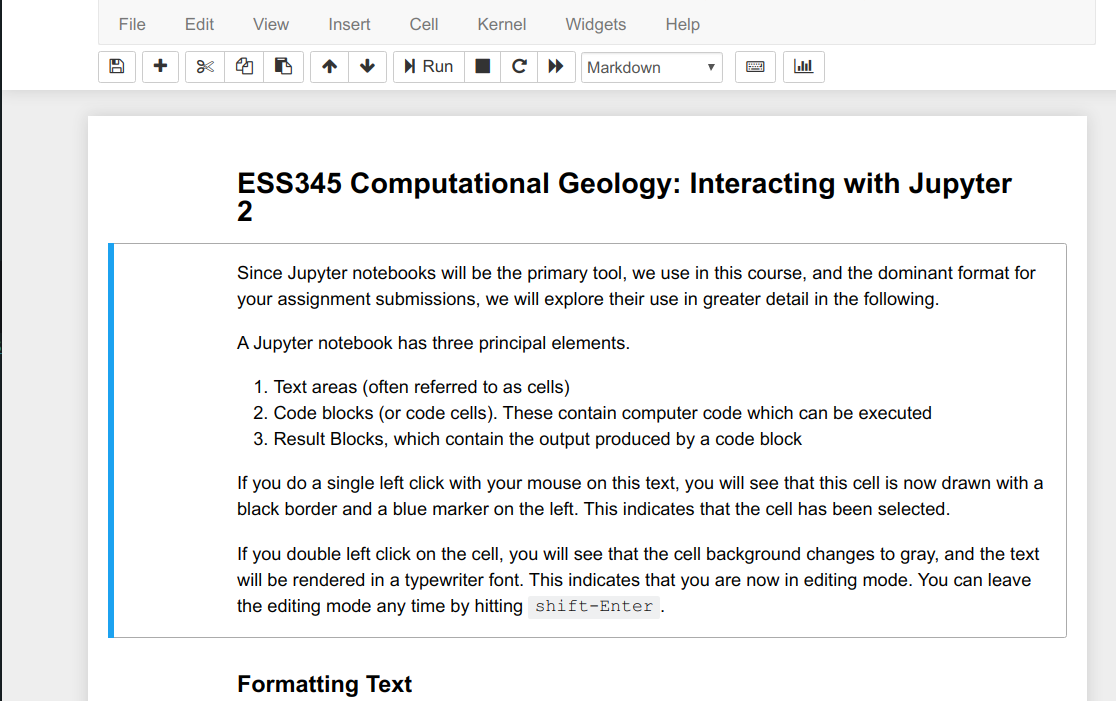
\includegraphics[width=0.7\textwidth]{./figures/Screenshot_20200527_133749.png}
\caption{\label{nbselected}A single click will select a notebook cell, which is indicated by the blue border to the left.}
\end{figure}


If you double-click on this cell, you will see that the cell
background changes to gray, rendering the text in a
typewriter font. This indicates that you are now in editing mode. You
can leave the editing mode any time by hitting \texttt{Shift-Enter}.
\begin{figure}[htbp]
\centering
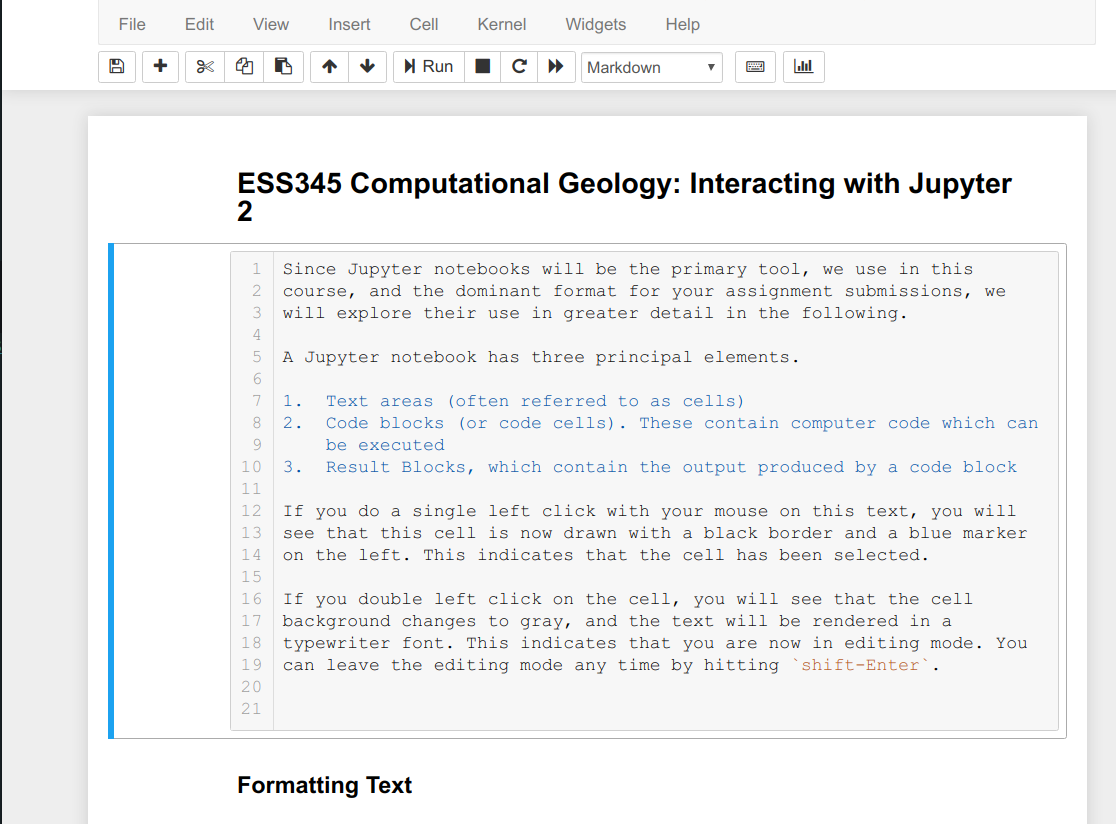
\includegraphics[width=0.7\textwidth]{./figures/Screenshot_20200527_133820.png}
\caption{\label{nbediting}A double click on any cell it will activate the editing mode. You can leave the editing mode any time by hitting \texttt{shift-Enter}.}
\end{figure}

Also, most of the usual keyboard shortcuts will work:
\begin{itemize}
\item Ctrl-z = undo
\item Ctrl-c = copy
\item Ctrl-x = cut
\item Ctrl-v = insert
\end{itemize}
\subsection{Potential Problems}
\label{sec:orgf207d61}
Sometimes, you may lose the connection to the Jupyter
server. This is indicated by the red \texttt{Not Connected} icon in the
status bar (see Fig.\ref{noconn}). This is usually caused by a firewall
rule. Please speak to a TA or the instructor to resolve this issue.
\begin{figure}[htbp]
\centering
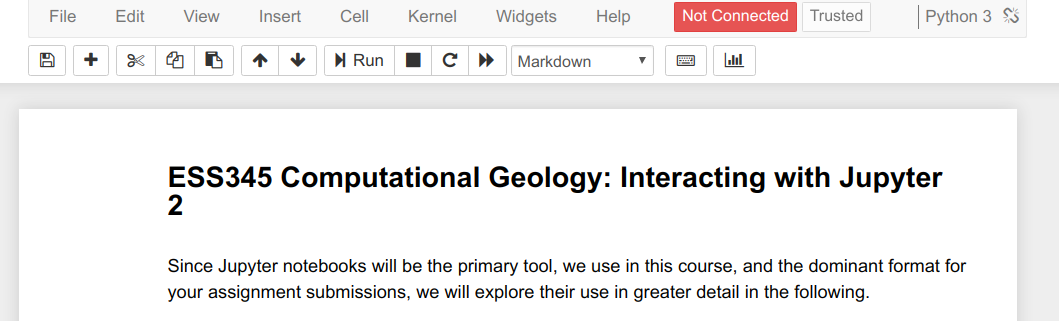
\includegraphics[width=0.7\textwidth]{./figures/Screenshot_20200527_134756.png}
\caption{\label{noconn}The red \texttt{not connected} icon indicates that you lost connection to your Jupyter Server. This is usually caused by a firewall rule. Please speak to a TA or the instructor to resolve this issue.}
\end{figure}
\subsection{Formatting Text}
\label{sec:org8b41fc5}
Before exploring how-to-use Jupyter notebooks to run python code,
let's explore how to format the text in the text cells. Create  a
new notebook in your \texttt{My\_stuff} folder. You can do this via the drop-down list called \texttt{New} in the upper right corner, and then select
\texttt{Python 3}, and rename the new file. These steps should now pose no
problem to you. If they do, please speak up!

Once your new notebook is open, it will look like
Fig. \ref{nbfirst}. Notice the text \texttt{In [ ]:} on the left side. This
tells you that this is a code cell that expects python code. So before
we start playing with text, we need to change the cell type (see Fig. \ref{celltype})
\begin{figure}[htbp]
\centering
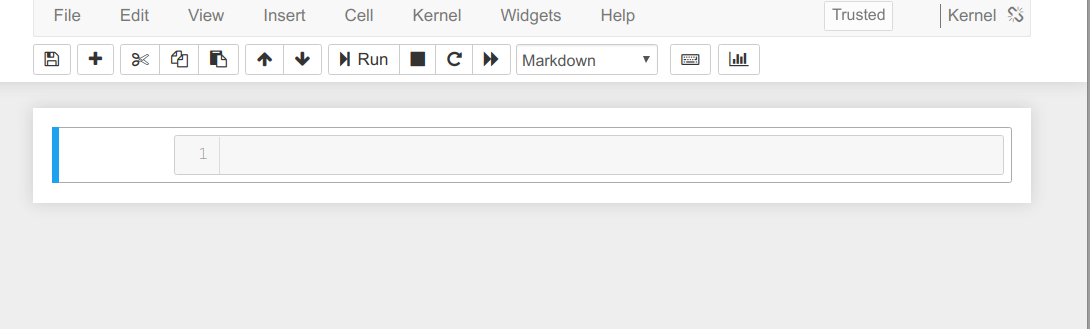
\includegraphics[width=0.7\textwidth]{./figures/Screenshot_20200527_145057.png}
\caption{\label{nbfirst}The default view when opening a new notebook. Note the text \texttt{In [ ]:} on the left side. This tells you that this is a code cell that expects python code.}
\end{figure}

Use the dropdown menu to change the cell type to \texttt{markdown}.
\begin{figure}[htbp]
\centering
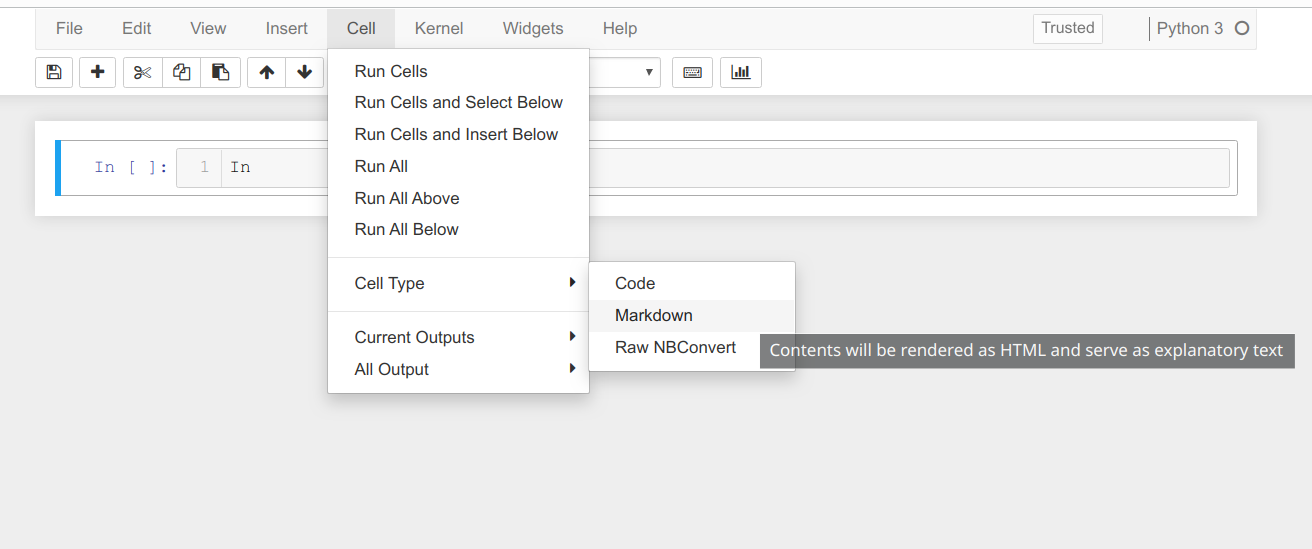
\includegraphics[width=0.7\textwidth]{./figures/Screenshot_20200527_150324.png}
\caption{\label{celltype}Use the dropdown menu to change the cell type to \texttt{markdown}}
\end{figure}


Once you have changed the cell to markdown, you will note that the \texttt{In
[ ]:} text on the left is now gone.

Next, copy the following lines into your new notebook cell:
\subsection{This is a second-level heading}
\label{sec:orge6fcbb4}

This is \textbf{bold} text

\begin{enumerate}
\item This is a simple list
\begin{itemize}
\item First list entry
\item Second list entry
\end{itemize}
\item This is the 3rd entry in the enumerated list and has no other
purpose than just being the 3rd entry.
\end{enumerate}

You will notice that the formatting has been lost. Go back to these
instructions, activate editing mode, and explore how to create the
formatting you see (see Fig.\ref{mdsyntax}) . Now go to your new
notebook, and apply the \texttt{mark down} syntax in your own notebook.
\index{Markdown Syntax}. Remember that you can leave the
edit mode any time by hitting \texttt{Shift+Enter}.

\begin{figure}[htbp]
\centering
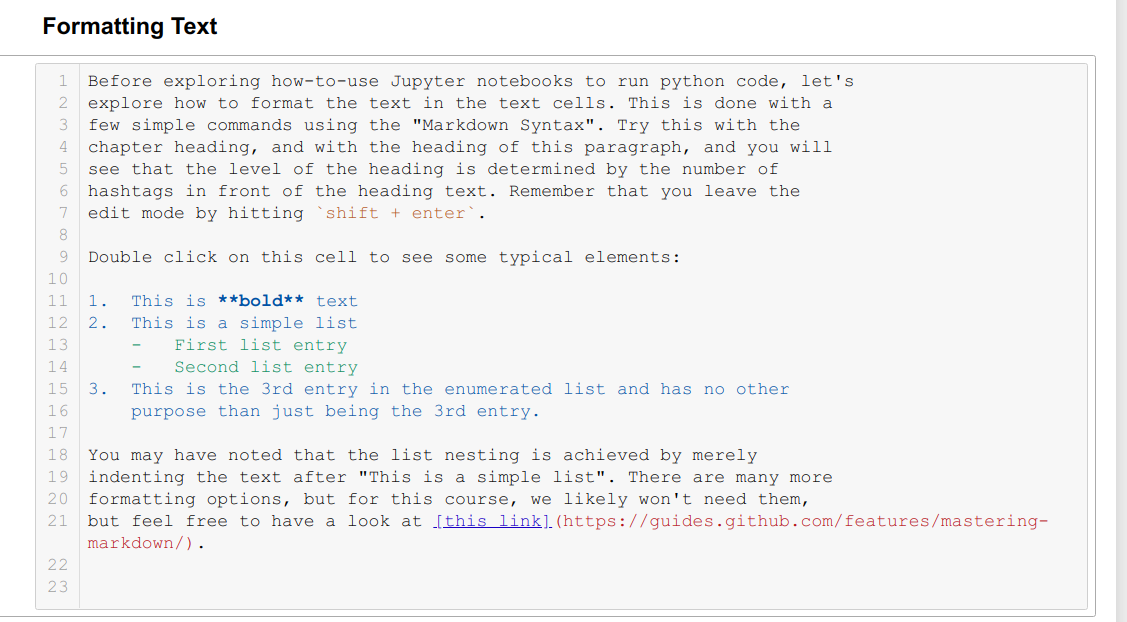
\includegraphics[width=0.7\textwidth]{./figures/Screenshot_20200527_153811.png}
\caption{\label{mdsyntax}Here, you can see how to format your text with \texttt{mark down} syntax}
\end{figure}


You may have noted that the list nesting is achieved by 
indenting the text after "This is a simple list". There are many more
formatting options, but for this course, we likely won't need them,
but feel free to have a look at \href{https://guides.github.com/features/mastering-markdown/}{this link}.

\textbf{Last but not least} save your edits by clicking on the floppy disk
icon in the upper left corner. This will create a checkpoint so that
you can return to this version at any time!
\subsection{Adding Code cells}
\label{sec:org1b1b8fe}
Now let's try adding a code cell below the text cell and enter a
trivial statement like \texttt{1 + 1} and hit \texttt{Shift+Enter} and you should
see the result displayed below the code cell (hopefully, it is
2). Go ahead and edit your code cell (e.g., 1+3) and hit \texttt{Shift+Enter}
again. The result should change accordingly (see Fig.\ref{codesnap})
\begin{figure}[htbp]
\centering
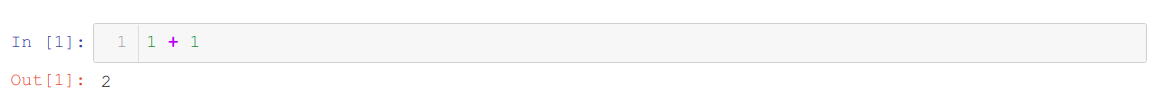
\includegraphics[width=0.7\textwidth]{./figures/Screenshot_20200527_161029.png}
\caption{\label{codesnap}Example of a trivial python statement}
\end{figure}

\textbf{Note that your edits are not auto-saved! You need to explicitly use the
floppy disk icon (leftmost, directly under \texttt{File}) to save your work!}
\subsection{Downloading your notebook}
\label{sec:org7b7fa27}
All of your assignments will have to be submitted on Quercus. In order
to mark your assignments, you need to submit a pdf copy, as well as
the actual notebook file. This is easily done via the \texttt{File} dialogue
(see Fig. \ref{fdialog})
\begin{figure}[htbp]
\centering
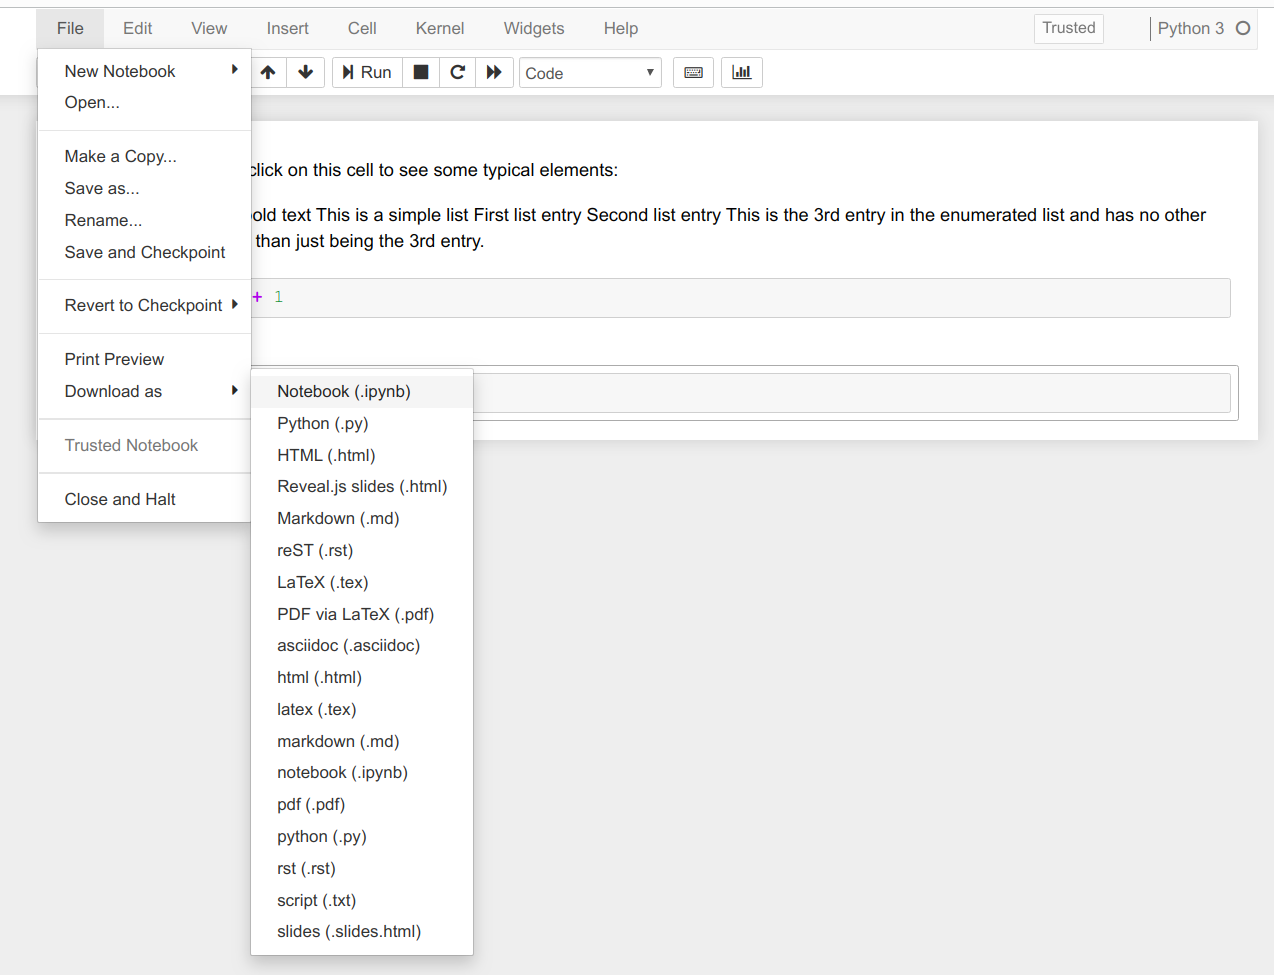
\includegraphics[width=0.7\textwidth]{./figures/Screenshot_20200527_161555.png}
\caption{\label{fdialog}You can download the notebook in a variety of formats.}
\end{figure}
\subsection{Recap}
\label{sec:org97659c7}
In this module, you learned how-to:

\begin{enumerate}
\item Create a notebook \index{notebook!creation}
\item Save a notebook \index{notebook!saving}
\item Download a notebook \index{notebook!download}
\item Create text cells  \index{notebook!create text cell}
\item Edit and format text cells  \index{notebook!text cell!edit}  \index{notebook!text cell!format}
\item Create code cells \index{notebook!code cell!create}
\item Execute code in a code cell  \index{notebook!code cell!execute}
\item Add a new code cell  \index{notebook!code cell!add}
\end{enumerate}
\end{document}